\section{Задачи}
\subsection*{Задача 1}
Предприятие через 6 лет желает иметь на счете 1600 тыс. руб. Для этого оно должно делать ежегодный взнос в банк по схеме пренумерандо. Определить размер ежегодного взноса, если банк предлагает 13\% годовых (проценты сложные).

\begin{center}
	Решение
\end{center}

По формуле наращения аннуитета имеем:
\[ FV(A) = A\dfrac{(1+E)^n - 1}{E} \times (1 + E) ;\]
\[ A = \dfrac{FV(A)}{\dfrac{(1+E)^n - 1}{E} \times (1 + E)} ;\]
\[ A = \dfrac{1600}{\dfrac{(1+0,13)^6 - 1}{0,13} \times (1 + 0,13)}; \]
\[ A = 170,13  \]

Ответ: размер ежегодного взноса по схеме пренумерандо составляет 170,13 тыс. руб.

\subsection*{Задача 2}
ОАО «Петя + Миша» имеет возможность профинансировать инвестиционный проект на 75\%  за счет заемного капитала и на 25\% за счет собственных средств. Средняя процентная  ставка за кредит составляет 11\%, цена собственного капитала 6\%. Доходность проекта планируется на уровне 15\%. Следует ли реализовать данный инвестиционный проект?

\begin{center}
	Решение
\end{center}

Доходность инвестиционного проекта должна превышать стоимость капитала. Для сравнения этих показателей, рассчитаем средневзвешенную стоимость капитала (WACC) и сравним полученное значение с уровнем доходности.
\[ WACC = 0,75 \times 11\% + 0,25 \times 6\%;\]
\[ WACC = 9,75\%.\]

Ответ: полученное значение средневзвешенной стоимости капитала 9,75\% ниже доходности 15\%, следовательно данный инвестиционный проект является целесообразным.


\subsection*{Задача 3}
По проекту стоимость годового выпуска продукции будущим предприятием должна составлять 100 млн. рублей, а затраты на 1 рубль товарной продукции --- 0,85 рублей. Проектный срок строительства объекта составляет 3 года. Определите проектную эффективность капитальных вложений, срок их окупаемости и как изменятся показатели эффективности капитальных вложений при условии сокращения срока  строительства на 3 месяца. Сметная стоимость строительства объекта 50 млн. руб.

\begin{center}
	Решение
\end{center}

Эффективность капитальных вложений --- соотношение между затратами на производство основных фондов и получаемыми результатами. Из условия вычислим проектную рентабельность предприятия:
\[ R = \frac{\text{Выручка}}{\text{Затраты}}; \]
\[ R = \frac{\text{100}}{\text{85}} = 1,1765; \]

Рентабельность предприятия составит 17,65\%.

Годовой доход (P) составляет: 100 -- 85 = 15 млн. руб.

Эффективность капитальных вложений:
\[ROI = \frac{P}{IC} ;\]
\[ROI = \frac{15}{50} = 0,3 \]
Срок окупаемости (T):
\[ T = \frac{IC}{P}; \]
\[ T = \frac{50}{15} = 3,33\  \text{г.} \]

\subsection*{Задача 4}
На основании исходных данных таблицы и вариантов ставки дисконта рассчитать  показатели эффективности: NPV; PI; DPP и сделать выводы о влиянии динамики денежного потока на показатели эффективности проектов. Ставка дисконта 30.

% Please add the following required packages to your document preamble:
% \usepackage{graphicx}
\begin{table}[!h]
	\small
	\caption{Характеристика инвестиционных проектов, млн.руб.}
	\label{my-label}
	\begin{tabularx}{\textwidth}{|K{3.25cm}|K{4cm}|K{4cm}|K{4cm}|}
			\hline
			Годы & Проект А & Проект Б & Проект В \\ \hline
			0    & -250     & -250     & -250     \\ \hline
			1    & 50       & 200      & 125      \\ \hline
			2    & 100      & 150      & 125      \\ \hline
			3    & 150      & 100      & 125      \\ \hline
			4    & 200      & 50       & 125      \\ \hline
		\end{tabularx}
\end{table}

\begin{center}
	Решение
\end{center}

Рассчитаем показатели эффективности для каждого проекта (см. таблицы 2--4).
	
Были получены следующие результаты. При ставке дисконта (30\%) наибольшую эффективность имеет проект Б с наиболее быстрым сроком окупаемости 2,16 года и и индексом доходности 1,223. Проект В имеет больший срок окупаемости 3,52 года и индекс доходности 1,084. Проект А оказался неэффективным, так как первоначальные инвестиции оказались больше дисконтированных денежных потоков от реализации проекта.

Так как наибольшую эффективность показал проект, в процессе реализации которого вложенные средства возвращаются быстрее, можно предположить, что более быстрый возврат вложенных средств имеет положительное влияние на показатели эффективности инвестпроектов.
%Рассчитаем NPV для проета А. Для этого найдем дисконтированный денежный поток.\\
%\[50 \cdot \dfrac{1}{(1+0,3)^1} = 38,5\]
%\[100 \cdot \dfrac{1}{(1+0,3)^2} = 59,2\]
%\[150 \cdot \dfrac{1}{(1+0,3)^3} = 68,3\]
%\[200 \cdot \dfrac{1}{(1+0,3)^4} = 70\]
%\[NPV = -250+38.5+59.2+68.3+70=-14\]
%
%Рассчитаем PI.
%\[PI = \dfrac{-14}{250}+1=-1.056\]

%Рассчитаем DPP.
%0 год: -250\\
%1 год: -211,5\\
%2 год: -152,3\\
%3 год: -84\\
%4 год: -14.

\begin{table}[!h]
	\caption{проект А}
	\label{project_A}
	\small
	\setlength{\extrarowheight}{1.2mm}
		\begin{tabularx}{\textwidth}{|K{1.12cm}|K{1.12cm}|p{8cm}|p{5cm}|}
		\hline
		&& \multicolumn{1}{c|}{$NPV$}                      & \multicolumn{1}{c|}{$DPP$} \\ \hline
		0 &$ -250$&                                                                   &  $    -250   $                 \\ \hline
		1 &$5$0& $50 \cdot \frac{1}{(1+0,3)^1} = 38,5$  &$ -250 +38,5   = -211,5     $            \\ \hline
		2 & $100$&$100 \cdot \frac{1}{(1+0,3)^2} = 59,2$ & $-211,5  +59,2=152,3      $           \\ \hline
		3 &$150 $&$150 \cdot \frac{1}{(1+0,3)^3} = 68,3$ &$-152,3  +68,3=-84    $             \\ \hline
		4 &$200$& $200 \cdot \frac{1}{(1+0,3)^4} = 70$  & $-84 +70= -14     $                \\ \hline
		&&$NPV = -250+38,+59,2+68,3+70=-14$     & $-14 $                     \\ \hline
		&&$PI = \frac{-14}{250}+1=-1,056$                                        & $DPP = $                 \\ \hline
		\end{tabularx}
		\end{table}

\begin{table}[!h]
	\label{project_B}
	\caption{проект Б}
	\small
	\setlength{\extrarowheight}{1.2mm}
	\begin{tabularx}{\textwidth}{|K{1.12cm}|K{1.12cm}|p{8cm}|p{5cm}|}
		\hline
		& &\multicolumn{1}{c|}{$NPV$}                      & \multicolumn{1}{c|}{$DPP$} \\ \hline
		0 & $-250$&                                                                   &  $    -250   $                 \\ \hline
		1 & $200$&$200 \cdot \frac{1}{(1+0,3)^1} = 153,9$  &$ -250 +153,9   = -96,1     $            \\ \hline
		2 & $150$&$150 \cdot \frac{1}{(1+0,3)^2} = 88,8$ & $-96,1  +88,8=-7,3      $           \\ \hline
		3 &$100$& $100 \cdot \frac{1}{(1+0,3)^3} = 45,5$ &$-7,3  +45,5=38,2    $             \\ \hline
		4 &$50$&$50 \cdot \frac{1}{(1+0,3)^4} =17,5$  & $38,2 +17,5= 55,7     $                \\ \hline
		&&$NPV = -250+38,+59,2+68,3+70=55,7$     & $55,7 $                     \\ \hline
		&&$PI = \frac{55,7}{250}+1=1,223$                                        & $DPP = 2,\frac{7,3}{45,5}=2,16$                 \\ \hline
	\end{tabularx}
\end{table}

\begin{table}[!h]
	\caption{проект В}
	\label{project_C}
	\small
	\setlength{\extrarowheight}{1.2mm}
	\begin{tabularx}{\textwidth}{|K{1.12cm}|K{1.12cm}|p{8cm}|p{5cm}|}
		\hline
		& &\multicolumn{1}{c|}{$NPV$}                    & \multicolumn{1}{c|}{$DPP$} \\ \hline
		0 &$-250$&                                                                     &  $    -250   $                 \\ \hline
		1 & $125$&$125 \cdot \frac{1}{(1+0,3)^1} = 96,2$ &$ -250 +96,2   =-153,8     $            \\ \hline
		2 & $125$&$125 \cdot \frac{1}{(1+0,3)^2} = 74$    & $-153,8  +74=-79,8      $           \\ \hline
		3 &$125$& $125 \cdot \frac{1}{(1+0,3)^3} = 56,9$ &$-79,8  +56,9=-22,9    $             \\ \hline
		4 & $125$&$125 \cdot \frac{1}{(1+0,3)^4} =43,8$  & $-22,9 +43,8= 20,9     $                \\ \hline
		&&$NPV = -250+96,2+74+56,9+43,8=20,9$     & $20,9 $                     \\ \hline
		&&$PI = \frac{20,9}{250}+1=1,084$               & $DPP = 3,\frac{22,9}{43,8}=3,52$                 \\ \hline
	\end{tabularx}
\end{table}

\newpage
\subsection*{Задача 5}
На приобретение мясоперерабатывающим предприятием новой технологической линией израсходовано 39 млн.руб.

Срок службы оборудования --- 5 лет. Амортизация начисляется линейным методом. Чистая прибыль за расчетный период прогнозируется по годам: 1-й --- 10 млн. руб., 2-й --- 12 млн. руб., 3-й --- 10 млн. руб., 4-й --- 10 млн. руб., 5-й --- 9 млн. руб. Цена капитала, инвестируемого в проект --- 25\%. Определите целесообразность приобретения новой  технологической линии на основе расчета внутренней нормы доходности проекта. Построить график зависимости NPV от ставки дисконта Е.

\begin{center}
	Решение
\end{center}

\begin{table}[!h]
	%\caption{}
	\label{meat}
	\small
	\setlength{\extrarowheight}{1.2mm}
	\begin{tabularx}{\textwidth}{|p{6.75cm}|K{1.2cm}|K{1.2cm}|K{1.2cm}|K{1.2cm}|K{1.2cm}|K{1.2cm}|}
\hline
\multirow{2}{*}{Показатели}                    										    	 & \multicolumn{6}{c|}{Денежный поток по шагам расчета} \\ \cline{2-7} 
																											    	   & 0           & 1            & 2              & 3            & 4               & 5      \\ \hline
Первоначальные инвестиции              										    	    & $-39$   &                &                 &               &                 &        \\ \hline
Амортизация                                      												        &              & $7,8     $&$ 7,8  $    & $7,8  $   & $7,8 $       & $7,8 $   \\ \hline
Чистая прибыль                                   											    	  &             &$ 10    $   & $12   $     & $10 $     &$ 10   $      & $9 $     \\ \hline
Чистый денежный поток                        									            &             & $17,8 $   &$ 19,8 $   &$ 17,8 $  &$ 17,8$      &$ 16,8  $ \\ \hline
Дисконт. мн-ль при $E=25\% $               								                 &              &$ 0.8 $     &$ 0.64 $    & $0.512 $ &$ 0.410$  & $0.328 $ \\ \hline
Чистый дисконтированный денежный поток           					  &$ -39 $  & $14,24 $  &$ 12,67 $  &$ 9,11  $ & $7,3  $     & $5,51 $  \\ \hline
Накопленный чистый дисконтированный денежный поток     & $-39 $  &$ -24,76 $& $-12,09 $ & $-2,98$  & $4,32  $   & $9,83  $ \\ \hline
	\end{tabularx}
\end{table}

При ставке дисконта $25\% \  NPV = 9,83$. Рассчитаем $IRR$ при помощи метода итераций.

%$E = 30\%\\
%CF_1 =13,69\\
%CF_2 =11,72\\
%CF_3 =8,1\\
%CF_4 =6,23\\
%CF_5 =4,53\\
%NPV = -39+13,69+11,72+8,1+6,23+4,53=5,27$
%
%$E = 35\%\\
%CF_1 =13,19\\
%CF_2 =10,86\\
%CF_3 =7,24\\
%CF_4 =5,36\\
%CF_5 =3,75\\
%NPV = -39+13,19+10,86+7,24+5,36+3,75=1,4$
%
%$E = 40\%\\
%CF_1 =12,71\\
%CF_2 =10,10\\
%CF_3 =6,49\\
%CF_4 =4,63\\
%CF_5 =3,12\\
%NPV = -39+12,71+10,10+6,49+4,63+3,12=-1,95$

\begin{table}[!h]
	\small
	\setlength{\extrarowheight}{1.2mm}
	\begin{tabularx}{\textwidth}{|p{5.22cm}|p{5.22cm}|p{5.22cm}|}
		\hline
		$E = 30\%$& $E = 35\%  $ & $E = 40\% $  \\ \hline
		$CF_1 =13,69 $&$ CF_1 =13,19$& $CF_1 =12,71 $\\ \hline
		$CF_2 =11,72$ & $CF_2 =10,86 $& $CF_2 =10,10$\\ \hline
		$CF_3 =8,1$ &$ CF_3 =7,24$ &$ CF_3 =6,49 $  \\ \hline
		$CF_4 =6,23$& $CF_4 =5,36 $ & $CF_4 =4,63  $   \\ \hline
		$CF_5 =4,53$&$ CF_5 =3,75 $ &$ CF_5 =3,12 $    \\ \hline
		$NPV = -39+13,69+11,72+8,1+6,23+4,53=5,27$   & $NPV = -39+13,19+10,86+7,24+5,36+3,75=1,4 $  &$ NPV = -39+12,71+10,10+6,49+4,63+3,12=-1,95$ \\ \hline
	\end{tabularx}
\end{table}
$$IRR = E_1 + \dfrac{NPV(E_1)}{NPV(E_1)-NPV(E_2)}\times(E_2 - E_1) $$

$$ IRR = 35 + \dfrac{1,4}{1,4+1,95}\times(40- 35) = 37,1$$

Построим график зависимости чистого дисконтированного дохода от ставки дисконтирования (рисунок \ref{fig:npvegr}).
\begin{figure}[!h]
	\centering
	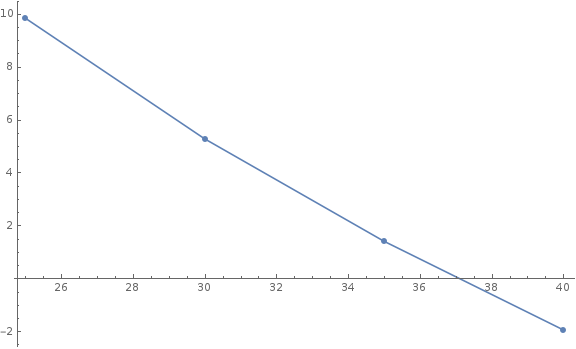
\includegraphics[width=1\linewidth]{npvegr}
	\caption{Зависимость NPV от ставки дисконта E}
	\label{fig:npvegr}
\end{figure}


Ответ: Проект является целесообразным, т.к. $IRR = 37,1$ выше стоимости капитала 25\%.
